\documentclass[border=10pt]{standalone}
\usepackage{pgfplots}
\pgfplotsset{width=7.5cm,compat=1.12}
\usepgfplotslibrary{fillbetween}
\pgfplotsset{compat=1.8}
\usepgfplotslibrary{fillbetween} %for fill under curve


\definecolor{dgrey}{rgb}{0,0,0}
\definecolor{hgrey}{rgb}{0,0,0}

\begin{document}

\newcommand{\zahl}[2]{
	\addplot[hgrey] plot coordinates { (0.25*#1,8) (0.25*#1,#2)};
	\addplot[dgrey, mark=*, mark size=1pt, only marks, small] coordinates {(0.25*#1,#2)};
}
    	
    	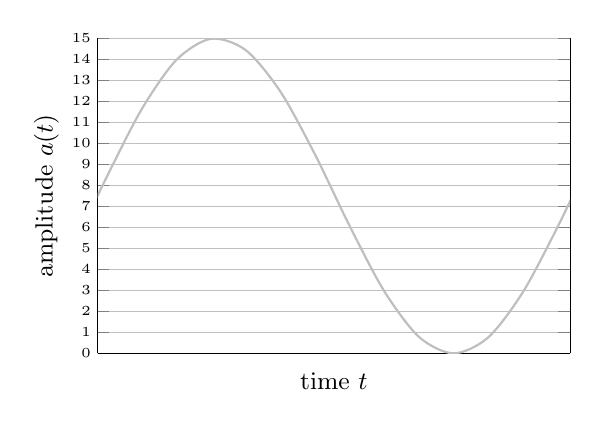
\begin{tikzpicture}

		\tiny
		\pgfplotsset{
			scale only axis,
		} 
	
			\begin{axis}[
				height= 4cm, width=6cm,
				xmin=0,xmax=0.25*25,
				xtick distance=7,				
				axis x line*=bottom,
				xticklabel= {~},
				xlabel = {\small time $t$},
				ylabel = {\small amplitude $a(t)$},
				grid,
				ymin=0, ymax=15,
				ytick distance=1,
				]
				
			\addplot [thick, black, smooth, domain=-4:7, color=lightgray] {7.5*sin(deg(x))+7.5};

%			
			\zahl{0}{8}
			\zahl{1}{9}
			\zahl{2}{11}
			\zahl{3}{13}
			\zahl{4}{14}
			\zahl{5}{15}
			\zahl{6}{15}
			\zahl{7}{15}
			\zahl{8}{14}
			\zahl{9}{13}
			\zahl{10}{12}
			\zahl{11}{10}
			\zahl{12}{8}
			
			\zahl{13}{7}
			\zahl{14}{5}
			\zahl{15}{3}
			\zahl{16}{2}
			\zahl{17}{1}
			\zahl{18}{0}
			\zahl{19}{0}
			\zahl{20}{0}
			\zahl{21}{1}
			\zahl{22}{2}
			\zahl{23}{4}
			\zahl{24}{5}
			\zahl{25}{7}	
	\end{axis}
				


    	\end{tikzpicture}%
    

\end{document}
